\section{Problem and formulation}
\label{sec:formulation}



\begin{figure*}[t]

  \centering
    \subfigure[]{
            \label{fig:pipeline:a}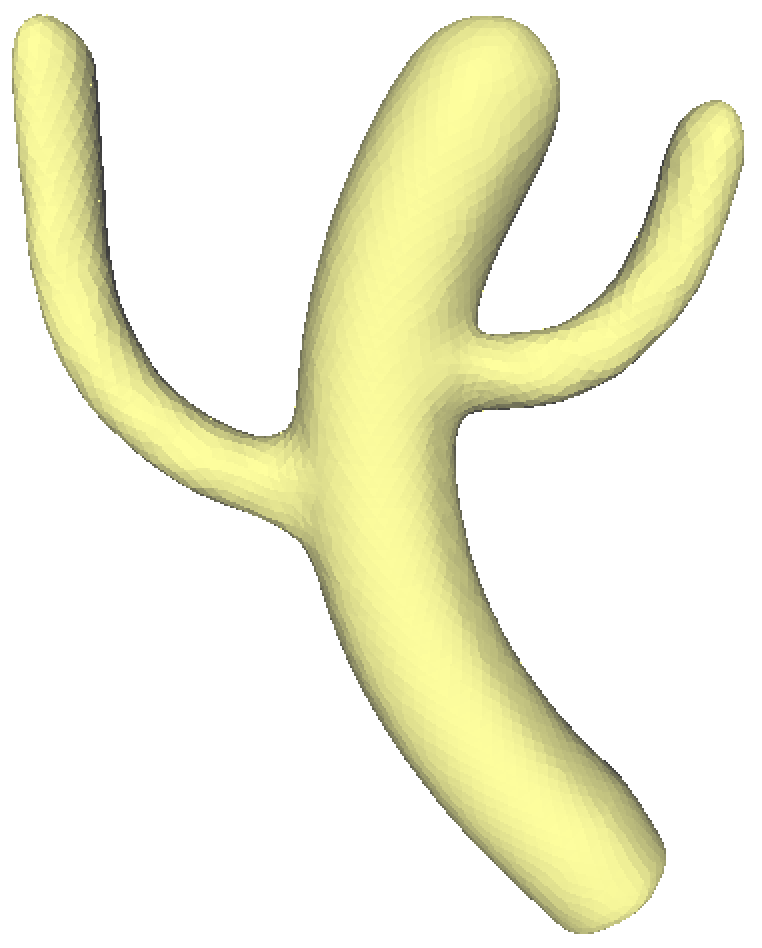
\includegraphics[width=.19\linewidth]{Figures/pipeline/1.png}}\quad
    \label{fig:pipeline:b}\subfigure[]{
            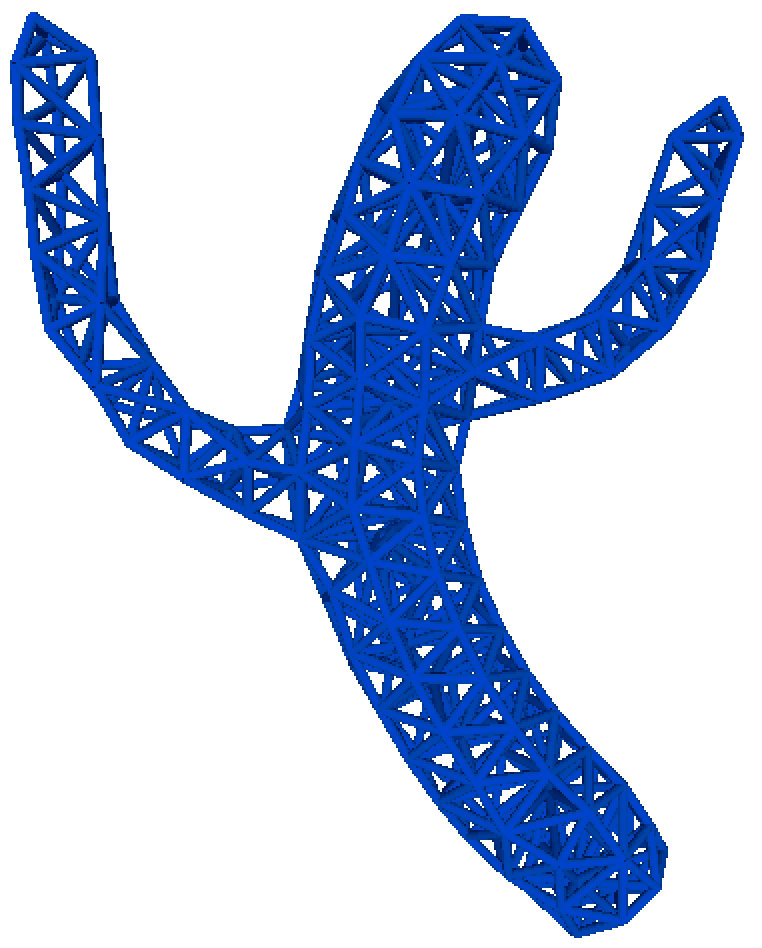
\includegraphics[width=.19\linewidth]{Figures/pipeline/2.png}
            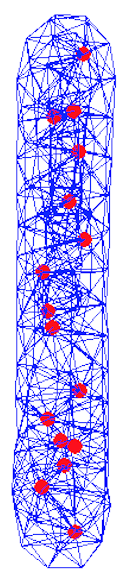
\includegraphics[width=.053\linewidth]{Figures/pipeline/m1.png}}\quad
    \label{fig:pipeline:c}\subfigure[]{
            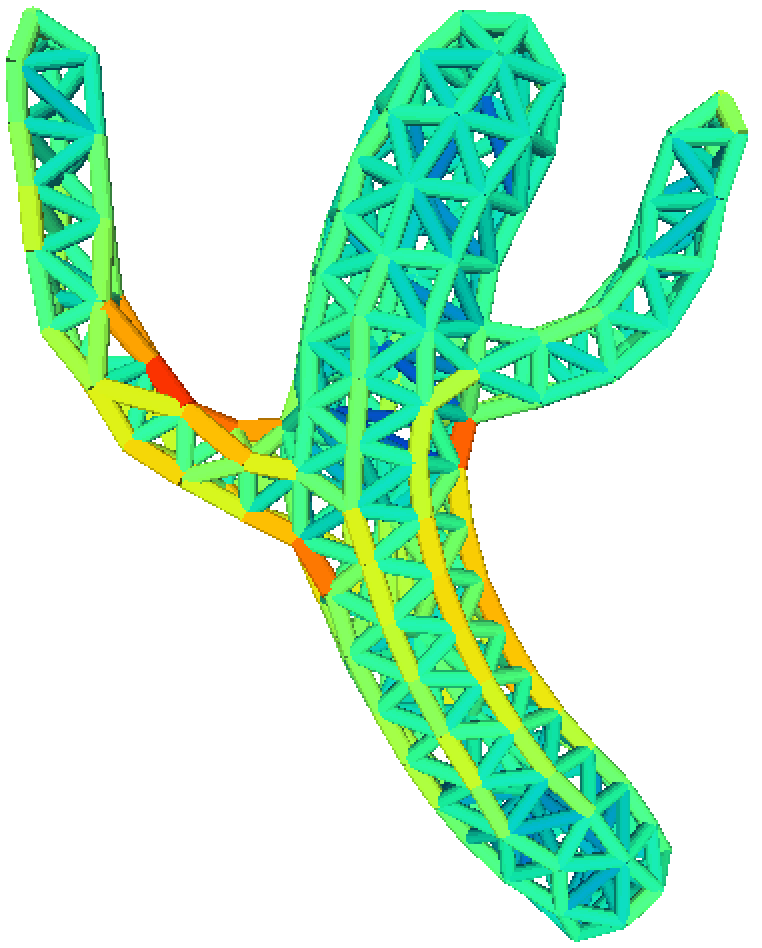
\includegraphics[width=.19\linewidth]{Figures/pipeline/3.png}
            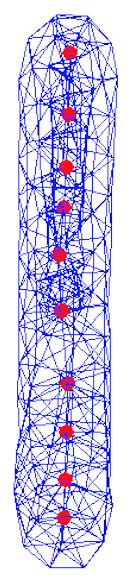
\includegraphics[width=.053\linewidth]{Figures/pipeline/m2.png}}\quad
    \subfigure[]{
            \label{fig:pipeline:d}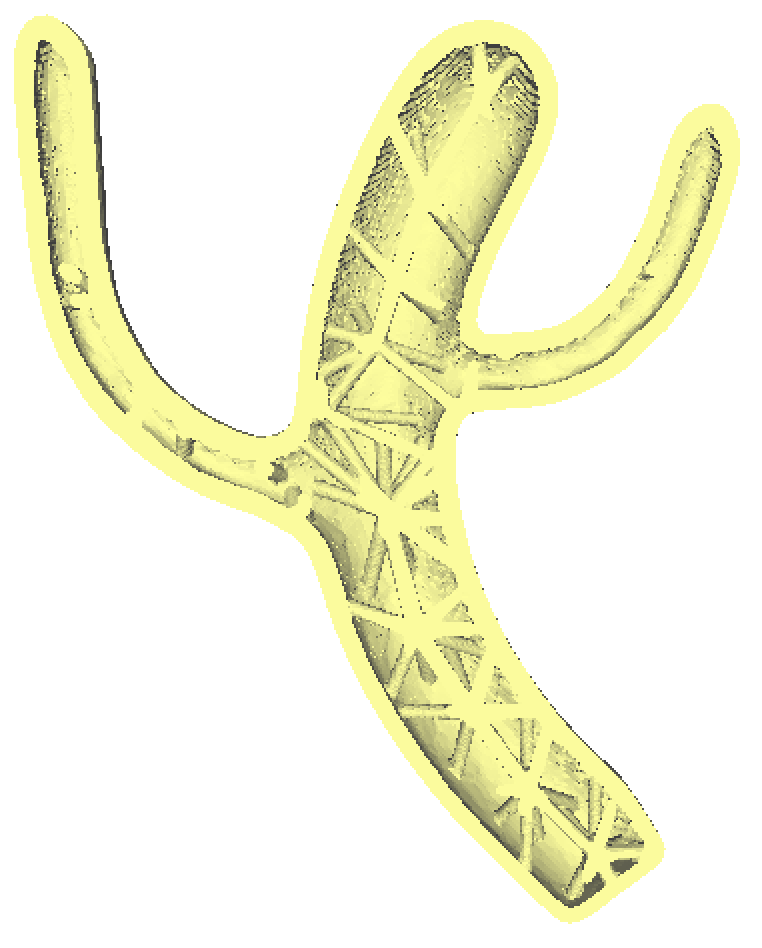
\includegraphics[width=.19\linewidth]{Figures/pipeline/4.png}}\quad

\caption{Pipeline of our approach. Given an input model (a), an initial frame structure (b) is generated. Our method runs a saddel point algorithm to obtain an optimized frame structure (c) which provides minimal deformation under unknown load distribution. (c) is colored to visualize their radii and a side view of the frame structure is presented to show the node position and topology connections before and after optimization. Then a post-processing step is applied to generate a solid structure (d) for 3D printing.
%
The front part of (d) is removed in order to show the internal structure.%Note that the beams in frame (c) have different radius and the shell of (d) is adaptive hollowed with different depth.
}
\label{fig:pipeline}
\end{figure*}



\noindent\textbf{Problem.}
The input of our framework is the surface mesh $S$.
%Assume the surface mesh $S$ of the input object is given.
Our goal is to generate an entity global stiffness object model $H$ consisting of an adaptive hollowed shell and a supportive interior sructure, while utilizing no more than a given amount of material. The generated object shares the same surface with as $S$ but has much less weight than $S$ for its lightweight supportive structure rather than solid filled.

\noindent\textbf{Remarks} The following two problems are usually considered in the structural optimization: Stiffness-to-Weight and Weight-to-Stiffness.
%%In the structural optimization field, researchers usually consider the following two problems:
Stiffness-to-Weight is to design a structure with the maximum stiffness using a specific amount of given material; and Weight-to-Stiffness is to design a structure with the least amount of material but satisfied the given stiffness expection. These two problems are dual and can be converted to each other by a simple binary search process. Without loss of generality, here we focus on the former one that takes the amount of material use as the constraint. We also consider the load is only from external forces as the internal forces, gravity for most of the time, remains very small compared with external forces so is ignored.



\subsection{Frame structure}
\label{subsec:frame}


%In the filed of fabrication engineering, an extensive attention has been paid to shape analysis and structural optimization [Crapo 1979; Crapo 1990; Rosenberg 1980; Haftka and Grandhi 1986].
%Many kinds of lightweight structures, including frame and honeycomb, have been developed to reduce weight and enforce strength~\cite{Kindinger:2001,wang:2013,buildtolast} during recent years.
%
%
%However, the vast majority of previous work focused on structural optimization and design under a given load environment like some specified forces.
%In real situation, an object might be handled or used in various possible ways, and specified forces cannot be exhaustive of all cases.
%As lacking of valid formulation for the above mentioned problem, traditional methods of structural optimization are unable to solve it efficiently.
%In this paper, the frame structure is proposed for not only being able to efficiently optimize but also formulating the adaptive hollowing and interior beams into a unified form.


%We adopt the frame structure~\cite{wang:2013} due to its ability of simulating the object, efficiency of optimizing the design, and the generation of the adaptive hollowing and interior lightweight supportive structure.
%The frame structure~\cite{wang:2013} is adopted here due to its ability to simulate the object, efficiently optimize the design, generate the adaptive hollowing and interior lightweight supportive structure into a unified form.



%formulating the adaptive hollowing surface shell and interior beams into a unified form as well as being able to efficiently optimize the design.
\parpic[r]{\label{fig:frame-structure}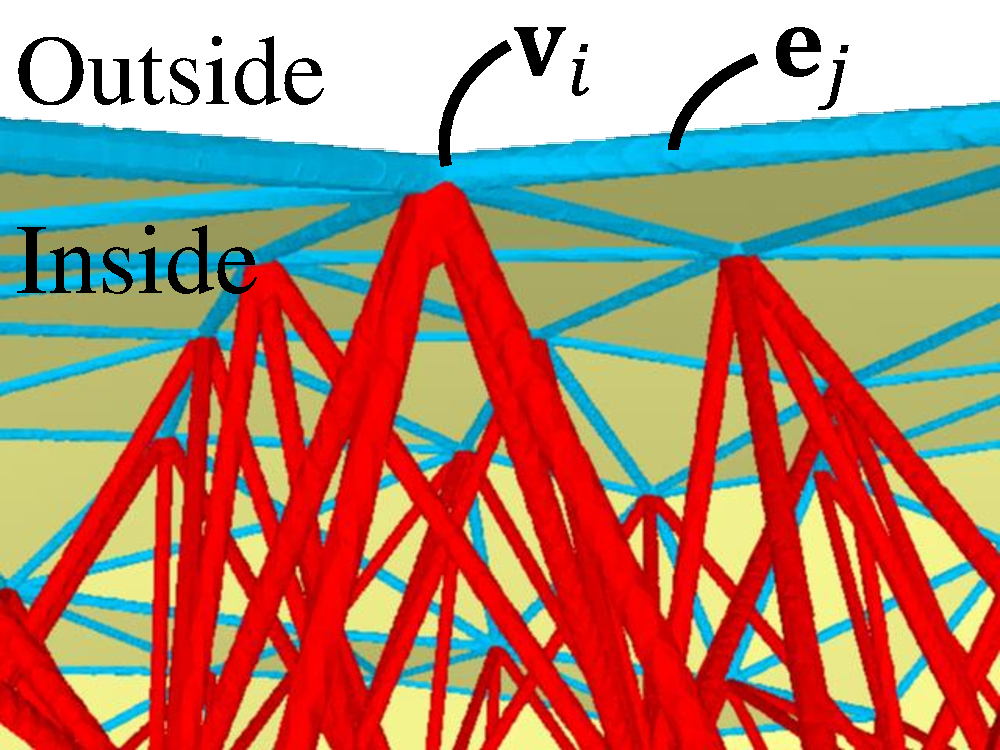
\includegraphics[width=0.2\linewidth]{Figures/structure/structure.pdf}}
%
A frame structure $\mathcal{T}$ consists of a set of frame nodes $V=\{\mathbf{v}_{i}, i=1,2,\cdots,m\}$ which are sampled on $S$ (marked in yellow) and in the volume enclosed by $S$, as well as a set of frame beams $E=\{\mathbf{e}_{j}, j=1,2,\cdots,n\}$ which are the edges connecting the nodes, as shown in the right figure.
%
Each node $\mathbf{v}_{i}$ represents a geometric position and each beam $\mathbf{e}_j$ is a cylindrical shape with radius $r_j$ and length $l_j$.
%
Here $\mathcal{T}$ can be seen as a graph of $V$ and $E$ with the geometry defining node positions, the beam radii, and the topology defining the connectivity between nodes.
%
For convenience, we also denote $V_S=\{\mathbf{v}_{i} \mid \mathbf{v}_{i}\in S\}$, $V_I=V\setminus V_S$,
$E_S=\{\mathbf{e}_j \mid \mathbf{e}_j\in S \}$ (marked in cyan), and $E_I = E\setminus E_S$ (marked in red).



%The frame structure~\cite{wang:2013} is adopted here due to formulating the adaptive hollowing surface shell and interior beams into a unified form
%as well as being able to efficiently optimize the design.
%%
%As shown in Figure~\ref{fig:frame-structure}\tuanfeng{a figure for frame structure}, a frame structure $\mathcal{T}$ consists of a set of frame nodes $V=\{\mathbf{v}_{i}, i=1,2,\cdots,m\}$ which are sampled on $S$ and in the volume enclosed by $S$, and a set of frame beams $E=\{\mathbf{e}_{j}, j=1,2,\cdots,n\}$ which are the edges connecting the nodes.
%%
%Each node represents a geometric position and each beam $\mathbf{e}_j \in E$ is a cylindrical shape with radius $r_j$ and length $l_j$.
%%
%Here $\mathcal{T}$ can be seen as a graph of $V$ and $E$ with the geometry defining node positions and beam radii, and the topology defining the connectivity between nodes.
%%
%For convenience, we also denote $V_S=\{\mathbf{v}_{i} \mid \mathbf{v}_{i}\in S\}$, $V_I=V\setminus V_S$,
%$E_S=\{\mathbf{e}_j \mid \mathbf{e}_j\in S \}$, and $E_I = E\setminus E_S$.



By taking adequate density of surface points, the appearance of frame $\mathcal{T}$ is expected to approximate $S$ within a certain geometric error \cite{yan2009isotropic}. After the frame is optimized, surface edges of frame (i.e., $E_S$) indicate the adaptive thickness (doubled radius) of the surface shell around the position of the edges.
Interior edges of the frame (i.e., $E_I$) are taken as cylinder-like supportive beams.
And then the frame $\mathcal{T}$ can be considered as a reasonable approximation of the final entity object $\mathcal{H}$.



%The frame structure is proposed for not only being able to efficiently optimize
%but also formulating the adaptive hollowing shell and interior beams into a unified form.



%Different from element-based methods for structural topology optimization where problems are expressed by element-wise step functions,
%the approach presented in this paper uses node positions and beam radii as design variables in the structural optimization.

The approach presented in this paper uses node positions and beam radii as design variables in the global stiffness structural optimization.
This is different from element-based methods for structural topology optimization~\cite{rozvany:2009}, where problems are expressed by tetrahedron-element-wise step functions.
%
As an effective discrete representation, the frame structure is fabrication-friendly and has simple mechanical properties which will be described in Section~\ref{subsec:mechanics}.



%
%\paragraph{Remark} When the optimization is finished, the optimized frame structure will guide on the solid generation. The interior structure is generated with a cylinder with the radii of an interior beam and the surface is adaptive hollowed with the depth equals to $\frac{2*(d_1*r_1+d_2*r_2+d_3*r_3)}{d_1+d_2+d_3}$, where $\{r_i,i=1,2,3\}$ is the radii of three most close beam with distance of $\{d_i,i=1,2,3\}$.
%


\subsection{Stiffness matrix}
\label{subsec:mechanics}


The mechanics of frame structure has been studied based on beam theory~\cite{Huges:1987,Gibson:1999,chandrupatla1991introduction} where frame beams are assumed to behave like simple beams under linear deformation caused by nodes' displacement or rotation. In our method, we make the following assumptions in calculating the equilibrium state of the structure.
\begin{itemize}
\item [a)] The beams are only connected to each other at nodes.
\item [b)] The beams are connected rigidly to have tensile, torsion, transverse shear force.
\item [c)] Each node has three displacement degrees of freedom and three rotation degrees of freedom.
\end{itemize}

\noindent\textbf{Linear relationship between deformation and force}
For a given frame structure, including both the surface and interior beams, the relationship between deformation \textemdash the displacement and rotation of each node, and the force (including torque) should satisfy the following discretized equilibrium equation.
\begin{equation} \label{eq:stiffness}
K(V,\mathbf{r}) D = F,
\end{equation}
where $V=(\mathbf{v}_1,\cdots,\mathbf{v}_m)$ also denotes the geometric positions of the nodes.
$K(V,\mathbf{r})$ is the stiffness matrix, which depends on node positions $V$ and beam radii $\mathbf{r}=(r_1,\cdots,r_n)$.
%
$F=(\mathbf{f}_1,\cdots,\mathbf{f}_m)^T$ is the force and torque distribution acting on each node and $D=(\mathbf{d}_1,\cdots,\mathbf{d}_m)^T$ is the displacement and the rotation of deformation caused by $F$.
For details, refer to~\cite{chandrupatla1991introduction}. Note that $F$ in Eq.~\eqref{eq:stiffness} is the sum of external force and only acts on a special set of nodes like $V_S$. This is for a better simulation of real world cases because external forces are always act on the surface.


\subsection{Eigen-Mode-like formulation}
%\subsection{Eigen-mode structural optimization}
\label{subsec:eigen-mode-opt}

Our global stiffness target, which minimizes the maximum deformation under unknown loads can be described as an Eigen-Mode-like formulation.

Originally, for the frame structure simulated from an object, we first find an external force $F$ that gives the maximal deformation. In order to avoid the scale problem, it is estimated by a deformation ratio $\frac{D^TD}{{F}^T{F}}$.
Then we minimize the maximal deformation ratio of the frame structure by varying the design variables $(V_I, \mathbf{r})$.


For an object in the state of equilibrium, the following conditions for $F$ are needed:
%
\begin{equation}
\label{cond-for-F}
\mathbf{1}\cdot F_i=0, \quad
 F_i \cdot (X_{i+1} -X_{c,i+1})-F_{i+1}\cdot (X_{i} -X_{c,i}) =0
\end{equation}
where $i=1,2,3$; $F_1,F_2,F_3$ are force components of $F$ along $x$, $y$, $z$ axis respectively; $X_1,X_2,X_3$
are the lists of $x$-, $y$-, $z$-coordinates of the nodes $X$ in a fame structure;
$X_{c}=(X_{c,1}, X_{c,2}, X_{c,3})$ is the center point of the object.
%
%\begin{equation}
%\label{cond-for-F}
%F_i = 0,\quad
% (F)_i \cdot (X_i -X_{c,i}) =0\quad (i=1,2,3)\:,
%\end{equation}
%where $\_1,\_2,\_3$ are force components along $x$, $y$, $z$ axis respectively; $X_1,X_2,X_3$
%are the lists of $x$-, $y$-, $z$-coordinates of the nodes $X$ in a fame structure;
%$X_{c}=(X_{c,1}, X_{c,2}, X_{c,3})$ is the centroid of the object. 
These two constrains indicate that both the force and the moment of the force are zero.
%As the upper bound of the amount of the material used is given, $G$ is a constant with two horizontal axis is zero.
%
%
%Also, for homogeneous Neumann boundary condition of $D$, the stiffness matrix
%$dK$ is singular. This is easy to seed since for a translation $D_0$ of object, $K D_0=0$.
%Moreover, let $R_0$ be the displacement vector from a rotation, we have $KR_0=0$.
%This fact also tells us that $\mbox{dim}(Null(K))=6$.
%
%
Since stiffness matrix $K$ is singular, for each $F$ satisfying Eq.~\eqref{cond-for-F}, to uniquely determine a solution $K D = F$, the translation and rotation should be ignored. Similiar to Eq.~\eqref{cond-for-F}, the total displacement and the total moment of displacement, the total rotation and the total moment of rotation are set to zero. Let the stiffness matrix under the above conditions on force and deformation be $\hat{K}$, which is now a regular matrix, then we have $D=\hat{K}^{-1}F$.
%

Thus, the structural optimization problem can be constructed as follows
\begin{equation} \label{eq:min-max-deformation}
\begin{array}{ccl}
\min\limits_{(V_I, \mathbf{r})\in\Theta} &
\max\limits_{F \mbox{ satisfying }  (\ref{cond-for-F}) } \frac{{(\hat{K}^{-1}F)}^T(\hat{K}^{-1}F)}{{F}^TF}
\end{array}
\end{equation}
where $\Theta$ is the collection of all feasible $V_I$ and $\mathbf{r}$; see detailed constrains in Sec.~\ref{subsec:constraints_for_opimization}.
%$$
%\min\limits_{(\mathbf{V}, \mathbf{r})\in\Theta}  \max \limits_{ \mathbf{1} \cdot F_i=0 } {(K^{-1}F)}^T(K^{-1}F)
%$$

\noindent\textbf{Eigen-Mode property} We here to discuss a more general situation if the external force can also act on $V_I$. As the stiffness matrix $\hat{K}$ is symmetric, the vector $F$ that maximizes the value ${{(\hat{K}^{-1}F)}^T(\hat{K}^{-1}F)}/{F^TF}$, accroding to \cite{Parlett:1998}, is just the eigenvector corresponding to the smallest eigenvalue of $\hat{K}$, denoted by $\lambda_{\min} (\hat{K})$ which is actually the same to the minimal positive eigenvalue of $K$.
%
Finally, we have such an eigen-mode optimization problem
\begin{equation}
\label{eq:max-min-eigenvalue}
\begin{array}{cl}
\max\limits_{(V_I, \mathbf{r})\in\Theta} & \lambda_{\min}^{*}(K(V,\mathbf{r}))
\end{array}
\end{equation}
where $\lambda_{\min}^{*}(K(V,\mathbf{r}))$ is the minimal positive eigenvalue of stiffness matrix $K(V,\mathbf{r})$.	


In this way, our formulation mathmatically proof the observation given by \cite{zhou:2013} that the eigenvector of kinematic equation indicates a structural worst-case. Here our linear relationship between deformation and force (ignored the first derivative of force) is a static but more realistic version of the kinematic equation. Our global stiffness optimization, therefore, can also be considered as automatically reinforce where the structure is the weakest. On the other hand, plenty of physical experiments done by \cite{zhou:2013} can also show that our deformation based formulation is reasonable in calculating 3D Printed object.


\subsection{ Constraints on structure design parameters}
\label{subsec:constraints_for_opimization}



\noindent\textbf{Radius bounds}
To make the frame structure printable, the radius of each beam should be no less than the minimum printable radius $\underline{r}$.
To avoid unrealistic design, an upper bound $\overline{r}$ for the radius is imposed for each beam.
Moreover, in order to retain the linear elastic property of the frame structure, the ratio between the length and the radius of a beam must satisfy the Euler buckling constraint.
%
In brief, the buckling and the printability can be integrated as a bounded constraint for each beam radius
\begin{equation} \label{eq:radius-bounds}
\underline{\eta}_j \leqslant {r}_j \leqslant \overline{r}, \quad  \mathbf{e}_j\in E,
\end{equation}
where $\underline{\eta}_j=\max(l_j/\alpha, \underline{r})$, $l_j$ is the length of beam $\mathbf{e}_j$, and $\alpha$ is the slenderness ratio.
%$\underline{r}$ is the minimum printable radius, and an upper bound $\overline{r}$.



%\if 0
%
%\paragraph{Buckling}
%%To validate the linear elastic property of frame, the ratio between the length and the radii of a beam should be constrained, which is known as Euler buckling and can be written as:
%%\begin{equation} \label{eq:buckling}
%%r_i \geqslant l_i / \alpha, \ \ \mathbf{e}_i \in E
%%\end{equation}
%%If the position of nodes are fixed, the buckling constrain can be considered as a lower buond of the radii of each beam.
%%
%In order not to fail the linear elastic property of frame structure,
%the ratio between length and radius of a beam must satisfy Euler buckling constraint
%\begin{equation} \label{eq:buckling}
%r_j \geqslant l_j / \alpha, \quad  \mathbf{e}_j \in E
%\end{equation}
%where $\alpha$ is the slenderness ratio.
%If the positions of nodes are fixed, the buckling constrain can be considered as a lower bound of the radius for each beam.
%
%\paragraph{Printability}
%To make the frame structure printable, the radius of each beam should be no less than the minimum printable radius $\underline{r}$.
%To avoid unrealistic design, we also set an upper bound $\overline{r}$ for each beam radius, i.e.,
%\begin{equation} \label{eq:printability}
%\underline{r}\leqslant {r}_j \leqslant \overline{r}, \quad  \mathbf{e}_j\in E.
%\end{equation}
%%
%%Note that both the buckling constraint and the printability constraint are imposed on the range of radius vector $\mathbf{r}$. For simplicity, we rewrite the constraint \eqref{eq:buckling} and \eqref{eq:printability} together as:
%%\begin{equation} \label{eq:lower_upper_r}
%%{r}_{j,lower} \leqslant {r}_j \leqslant {r}_{j,upper}, \quad \ \mathbf{e}_j\in E.
%%\end{equation}
%%where ${r}_{j,lower} = maximal(\underline{\eta},l_i / \alpha)$ and ${r}_{j,upper} = \overline{\eta}$.
%%
%For simplicity, the buckling~\eqref{eq:buckling} and the printability~\eqref{eq:printability} can be integrated into a range constraint of radius for each beam
%\begin{equation} \label{eq:radius-bounds}
%\underline{\eta}_j \leqslant {r}_j \leqslant \overline{r}, \quad  \mathbf{e}_j\in E.
%\end{equation}
%where $\underline{\eta}_j=\max(l_j/\alpha, \underline{r})$.
%
%\fi




\noindent\textbf{Volume}
%
The proposed problem is defined as optimizing the frame structure when a certain amount of material is given.
%
\parpic[r]{\label{fig:covered-area}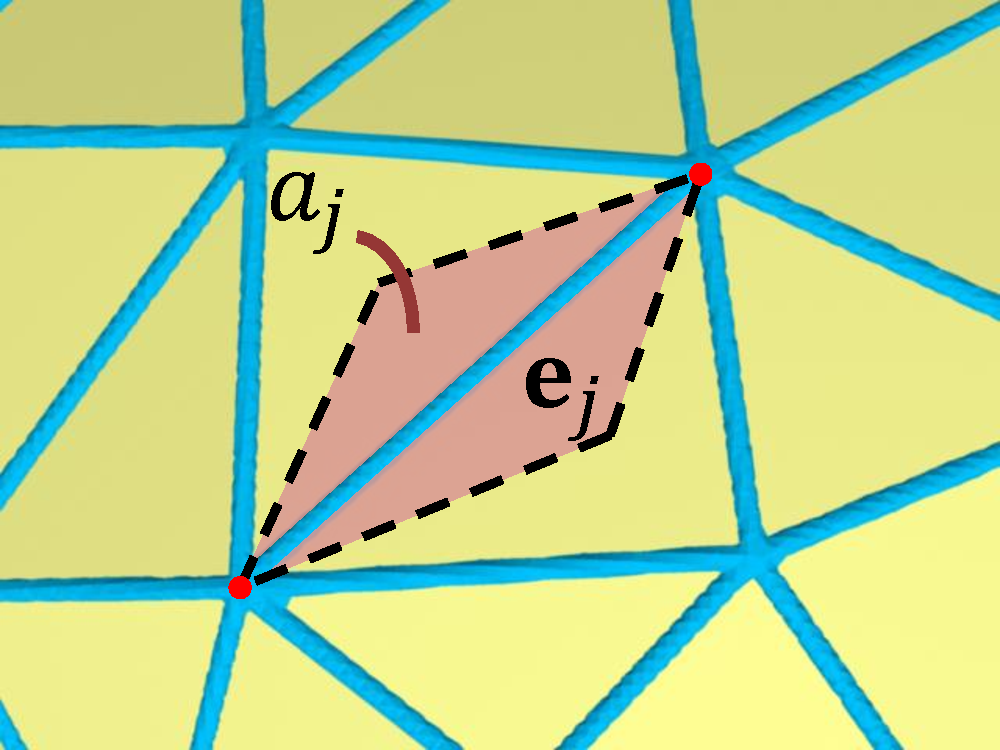
\includegraphics[width=0.2\linewidth]{Figures/area/area.pdf}}
Let $\overline{\mathrm{Vol}}$ be the amount of material available.
%Denote $\Omega$ the volume of solid material in designed structure $\mathcal{H}$.
%\parpic[r]{\label{fig:covered-area}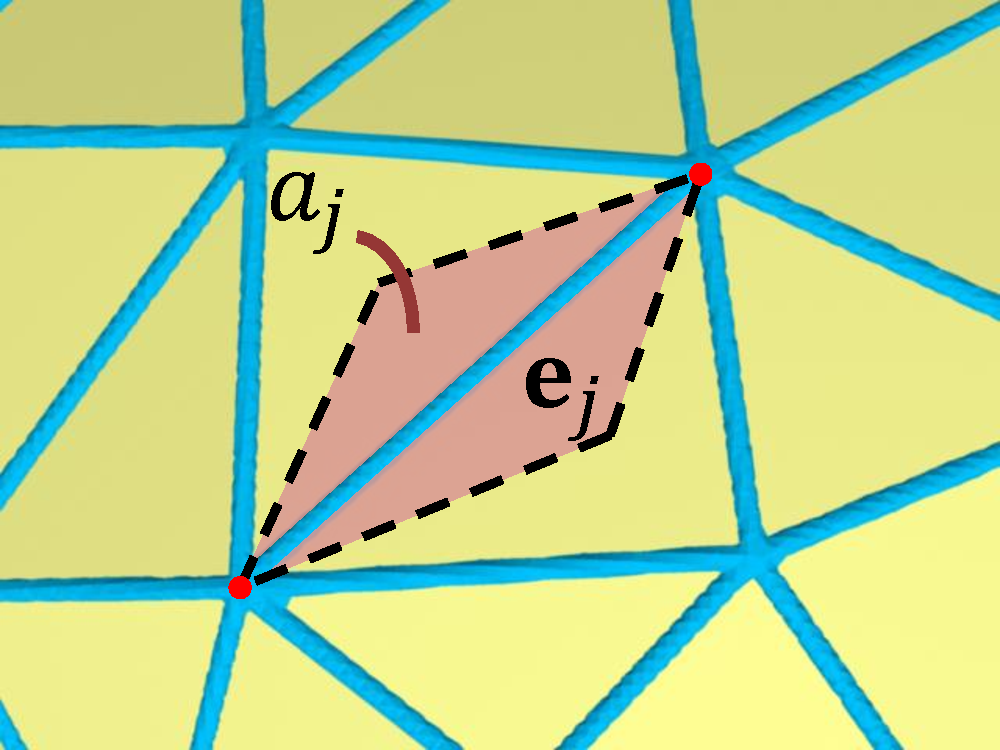
\includegraphics[width=0.4\linewidth]{Figures/area/area.pdf}}
The volume of solid material in the designed structure $\mathcal{H}$ consists of two parts:
the volume of interior beams in the frame, and the volume of adaptive-hollowed shell, which can be approximately calculated as
the sum of the product of the area covered by a surface beam and its doubled radius.
%
Thus we have a constraint on the material volume
\begin{equation} \label{eq:volume}
\sum_{\mathbf{e}_j\in E_I} \pi {r_j}^2 l_j + \sum_{\mathbf{e}_j\in E_S} 2 r_j a_j  \leqslant \overline{\mathrm{Vol}},
\end{equation}
where $a_j$ is the area covered by beam $\mathbf{e}_j$ on the surface.
In practice, $a_j$ is roughly calculated as the shaded area shown on the right.



%
%\[
%\Theta = \big\{ (\mathbf{V}, \mathbf{r}) \mid \ \mathrm{s.t.}\ \  \eqref{eq:radius-bounds}, \  \eqref{eq:volume} \big\}
%\]



%Overall, it's obvious that the most important constraint for the proposed problem is the total material cost, namely the volume upper bound $\overline{\Omega}$ of the solid $\mathcal{H}$.
%The volume of the solid consists of two parts: volume of interior structure, which is the same as the volume of interior beams of the frame, and the volume of adaptive-hollowed surface solid which can be approximately calculated as the sum of product of the area covered by a surface strframe edge 'covers' and doubled radii of the edge.\tuanfeng{figure}
%\begin{equation} \label{eq:volume}
%\sum_{\mathbf{e}_j\in E_1} \pi {r_i}^2 l_i + \sum_{\mathbf{e}_j\in E_2} 2r_i S_i  \leqslant \widetilde{\mathrm{Vol}}
%\end{equation}
%$S_i$ is the area which $i$th edge is coverd on the surface. In practice, we approximate $S_i$ with  $1/3$ of the are of the two triangles $\mathbf{e}_{i}$ attached.

\noindent\textbf{Shape barrier} The appearance of our optimal result should be the same with the surface of the input mesh. As a result, elements in internal beams set $E_I$ have to be kept inside of the volume enclosed by $S$. Many algorithms have been developed for this purpose. In our implementation, an efficient but approximate method is adapted that several test points are sampled from each beam for a quick check whether they are inside $S$. A feasable solution of the optimization problem is subject to the constraint that all the test points are inside $S$.



\noindent\textbf{Other constrains} The objective function of our optimization is very flexible and can be solved efficiently. As a result, addition constrains are able to be considered in our formulation such as stability, self-supportiveness, orientation, angle of beams, etc., including printability constrains specified by certain printing techniques. In this paper, we focus on the main problem \textendash \ global stiffness formulation, as these constrains have been well studied by many previous work~\cite{wang:2013}. 




%
%\begin{itemize}
%\item \textbf{Balance} For some standing objects, the center of mass of the output solid should be projected into the base of support\cite{prevost:2013}, which is easy to impose on the frame approximation with the same math form.
%\item \textbf{...}
%\end{itemize}




%
%
%\subsection{Eigen-mode structural optimization}
%\label{subsec:eigen-mode-opt}
%
%
%The problem at hand is defined as finding a frame structure which has the maximum global stiffness when a certain amount of material is given.
%In this section, we formulate the structural optimization problem that gives an optimal structure for all kind of force distribution by using eigen-mode analysis.
%For a frame structure of object, we first find a normalized  force $F$ (i.e., $\|F\|_{l^2}=1$) that maximizes
%the deformation $K^{-1}F$, which is estimated by $ \|K^{-1}F\|_{l^2} $.
%Then we optimize the maximal deformation of frame structure by varying the design variables $(V, \mathbf{r})$.
%
%Notice that since we are considering an equilibrium state, the following constraint conditions are needed:
%$$\mathbf{1}\cdot F_i=0,\quad (i=1,2,3)$$
%where $F=(F_1,F_2,F_3)$ are force components along $x, y, z$ coordinates respectively.
%Also, for homogeneous Dirichlet boundary condition of $D$, the stiffness matrix
%$K$ is singular, which is easy to see since for a translation $D_0$ of object, $K D_0=0$.
%This fact also tells us that $\mbox{dim}(Null(K))=3$. Thus, we append an constraint condition to $D$; for example,
%\begin{itemize}
%\item [a)] $\mathbf{1}\cdot  D=0$;
%\item [b)] $D=0$ for certain node.
%\end{itemize}
%With such a condition a) or b), there exists a unique $D$ for each $F$ that $\mathbf{1}\cdot F_i=0$ ($i=1,2,3$).
%In our model, to formulate an eigen-prolem, we choose the condition a).
%
%Since
%$(D+D_0)^T(D+D_0)=D^TD +D_0^TD_0$ for constant vector $D_0$, we know that each constraint condition of a) and b) gives the same shape of $D$, except for a shift, that maximizes $D^TD$.
%
%Thus, the structural optimization problem can be constructed as follows
%\begin{equation} \label{eq:min-max-deformation}
%\begin{array}{ccl}
%\min\limits_{(V, \mathbf{r})\in\Theta} &
%\max\limits_{\mathbf{1}\cdot F_i=0} {(K^{-1}F)}^T(K^{-1}F)
%\end{array}
%\end{equation}
%where $\Theta=\big\{(V, \mathbf{r}) \mid \ \text{subject to}\  \eqref{eq:radius-bounds} \ \text{and}\  \eqref{eq:volume}\big\}$.
%%$$
%%\min\limits_{(\mathbf{V}, \mathbf{r})\in\Theta}  \max \limits_{ \mathbf{1} \cdot F_i=0 } {(K^{-1}F)}^T(K^{-1}F)
%%$$
%Notice that the vector $F$ that maximizes the value  ${(K^{-1}F)}^T(K^{-1}F)$ is just the eigenvector
%corresponding to the largest eigenvalue of $K^{-T}K^{-1}$, denoted by $\lambda_{\max}(K^{-T}K^{-1})$.
%As $K$ is a symmetric matrix, $K^{-T}K^{-1}$ and $K$ have the same eigenvectors and the relationship of their eigenvalues by
%$$
%\lambda(K^{-T}K^{-1})=\dfrac{1}{\lambda(K)^2}.
%$$
%%Moreover, the eigenvector of $K$ with the constraint $a)$ or $b)$ is just the non-constant eigenvecotr of $K$ without constraint conditions.
%Thus, the force vector that maximizes ${(K^{-1}F)}^T(K^{-1}F)$ is given by the eigenvector of matrix $K$ corresponding to its smallest eigenvalue, denoted by $\lambda_{\min} (K)$, and reaches the maximum value of objective function as $\lambda_{\max}(K^{-T}K^{-1})=1/{\lambda_{\min}(K)^2}$.
%
%In practical computation, we can construct the stiffness matrix without constraint condition for $D$ and $F$ to
%obtain $\hat{K}$. Then, it is easy to see that the $\lambda_{\min} (K)$ is the minimal positive eigenvalue of $\hat{K}$.
%
%
%As a summary, we have such an eigen-mode optimization problem
%%$$
%%\max\limits_{(\mathbf{V}, \mathbf{r})\in\Theta}   \lambda_{\min} (K)
%%$$
%\begin{equation}
%\label{eq:max-min-eigenvalue}
%\begin{array}{cl}
%\max\limits_{(V, \mathbf{r})\in\Theta} & \lambda_{\min}^{*}(K(V,\mathbf{r}))
%\end{array}
%\end{equation}
%where $\lambda_{\min}^{*}(K(V,\mathbf{r}))$ is the minimal positive eigenvalue of stiffness matrix $K(V,\mathbf{r})$.
%


%\xuefeng{My revision ends here.}

%
%
%The problem at hand is defined as finding an almighty frame structure which has the maximum global stiffness
%under any unprescribed loads when a certain amount of material is given.
%%
%A frame structure with maximum global stiffness provides a minimum mean compliance for the worst-case (most-damaged) loads.
%%A frame structure with maximum global stiffness provides a minimum for the external work with the real displacement field or minimum mean compliance.
%%
%Since minimization of mean compliance is equivalent to the maximization of the total potential energy,
%the almighty structural optimization problem can be constructed as follows
%%(Hassani and Hinton 1999; Bendsoe and Sigmund 2003)%
%%
%\begin{equation} \label{eq:min-max-deformation}
%\begin{array}{ccl}
%\max\limits_{(\mathbf{V}, \mathbf{r})\in\Theta} &
%\min\limits_{\mathbf{D}\in\Pi} & \mathbf{D}^T \mathbf{K}(\mathbf{V},\mathbf{r})\mathbf{D}
%\end{array}
%\end{equation}
%where $\mathbf{D}\in\Pi = \big\{ \mathbf{D} \mid   \|\mathbf{D}\|_2=1,\sum\limits_{i=1}^m \mathbf{d}_i =\mathbf{0},\sum\limits_{i=1}^m \mathbf{v}_i\times\mathbf{d}_i =\mathbf{0} \big\}$ is the real displacement field,
%$\mathbf{D}^T \mathbf{K}(\mathbf{V},\mathbf{r})\mathbf{D}$ is total potential energy,
%and $(\mathbf{V},\mathbf{r})\in\Theta=\big\{(\mathbf{V}, \mathbf{r}) \mid \ \text{subject to}\  \eqref{eq:radius-bounds} \ \text{and}\  \eqref{eq:volume}\big\}$ are design variables in the frame structure.
%%
%Note that minimization of the total potential energy in~\eqref{eq:potential-energy-max} according to constrained $\mathbf{D}$
%is equivalent to satisfying the state equilibrium.
%%
%In the almighty structural optimization, the goal can be thought of as determination of optimal design variables
%to achieve the best load-bearing performance under any possible deformation.
%
%
%%\[
%%\Pi = \big\{ \mathbf{D} \mid   \|\mathbf{D}\|_2=1,
%%\sum\limits_{i=1}^m \mathbf{d}_i =\mathbf{0},\sum\limits_{i=1}^m \mathbf{v}_i\times\mathbf{d}_i =\mathbf{0} \big\}
%%\]
%%
%%\[
%%\Theta = \big\{ (\mathbf{V}, \mathbf{r}) \mid \ \text{subject to}\  \eqref{eq:radius-bounds} \ \text{and}\  \eqref{eq:volume} \big\}
%%\]
%
%
%
%In fact, the stiffness matrix $\mathbf{K}(\mathbf{V},\mathbf{r})$ is positive-semidefinite.
%The optimization of~\eqref{eq:potential-energy-max} can be reformulated as to maximizing the minimum non-zero eigenvalue of stiffness matrix, i.e.,
%\begin{equation}
%\label{eq:max-min-eigenvalue}
%\begin{array}{cl}
%\max\limits_{(\mathbf{V}, \mathbf{r})\in\Theta} & \lambda_{\min}^{*}(\mathbf{K}(\mathbf{V},\mathbf{r}))
%\end{array}
%\end{equation}
%where $\lambda_{\min}^{*}(\mathbf{K}(\mathbf{V},\mathbf{r}))$ represents the minimum non-zero eigenvalue of $\mathbf{K}(\mathbf{V},\mathbf{r})$.
%%
%Note that the constraints of deformation displacement field $\mathbf{D}$ have been implicitly passed on to the minimum non-zero eigenvalue of stiffness matrix.

